
\documentclass{beamer}
\usepackage[utf8]{inputenc}
\usetheme{focus} % Use the Focus theme supplied with the template
% Add option [numbering=none] to disable the footer progress bar
% Add option [numbering=fullbar] to show the footer progress bar as always full with a slide count

% Uncomment to enable the ice-blue theme
\definecolor{main}{RGB}{50, 97, 133}
\definecolor{background}{RGB}{240, 247, 255}

%------------------------------------------------

\usepackage{booktabs} % Required for better table rules
\usepackage{subcaption}
\usepackage{multirow}

%----------------------------------------------------------------------------------------
%	 TITLE SLIDE 
%----------------------------------------------------------------------------------------

\title{Word Count Problem \& \\Cross Correlation Calculation}

\subtitle{Based on MPI}

\author{Filipe Pires | 85122 | filipesnetopires@ua.pt \\ João Alegria | 85048 | joao.p@ua.pt}

\institute{University of Aveiro, DETI}

\date{\today}

%------------------------------------------------

\begin{document}

%------------------------------------------------

\begin{frame}
	\maketitle % Automatically created using the information in the commands above
\end{frame}

%----------------------------------------------------------------------------------------
%	 WORD COUNT
%----------------------------------------------------------------------------------------

\begin{frame}{Word Count Problem: Multi-Thread Mapping}
	The team efforts were focused on mapping the initial single-threaded implementation of the program to a multi-threaded environment.
	The required mapping was:
	\begin{itemize}
		\item A shared memory space would keep track of the files to be processed.
		\item Each worker thread would ask the shared memory for a chunk of text, process it and return the results to the shared memory.
		\item The shared memory would manage the files' content internally, enabling the distribution of chunks of text.
		\item The shared memory would keep track of all received results, enabling a print in the end of the global results processing of each file given as input.
	\end{itemize}
\end{frame}

%------------------------------------------------

\begin{frame}{Solution Diagram \& Entity Interaction}
	\begin{figure}
		\begin{subfigure}{.49\textwidth}
			\hspace*{-.3in}
			\includegraphics[width=1.2\linewidth]{wordCountDiagram.png}
			\caption{Solution Diagram}
			\label{wordDiagram}
		\end{subfigure}
		\begin{subfigure}{.49\textwidth}
			\hspace*{.1in}
			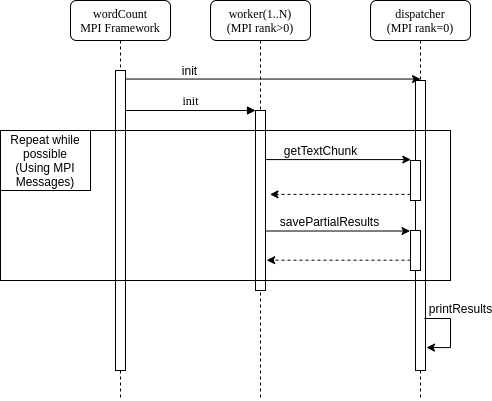
\includegraphics[width=1.05\linewidth]{wordCountInteraction.png}
			\caption{Entity Interactions}
			\label{wordInteraction}
		\end{subfigure}
	\end{figure}
\end{frame}

%------------------------------------------------

%----------------------------------------------------------------------------------------
%	 CROSS CORRELATION CALCULATION
%----------------------------------------------------------------------------------------

\begin{frame}{Cross Correlation Problem: Multi-Thread Mapping}
	Once again, our task was to map a single-threaded implementation of the solution for this second problem, previously developed by us, to a multi-threaded
	version of such implementation.
	The required mapping was:
	\begin{itemize}
		\item A shared memory space would keep track of the files to be processed.
		\item Each worker thread would ask the shared memory for the values of a signal and a specific $\tau$, calculate the cross correlation and return the results to the shared memory.
		\item The shared memory would manage the files' content internally, enabling the distribution of the same signals but with different $\tau$ values.
		\item The shared memory would keep track of all received results, enabling the program to write the results in the end of each file or to print them to the console.
	\end{itemize}
\end{frame}

%------------------------------------------------

\begin{frame}{Solution Diagram \& Entity Interaction}
	\begin{figure}
		\begin{subfigure}{.49\textwidth}
			\hspace*{-.3in}
			\includegraphics[width=.95\linewidth]{crossCorrelationDiagram.png}
			\caption{Solution Diagram}
			\label{crossDiagram}
		\end{subfigure}
		\begin{subfigure}{.49\textwidth}
			%\hspace*{.1in}
			\includegraphics[width=1.1\linewidth]{crossCorrelationInteraction.png}
			\caption{Entity Interactions}
			\label{crossInteraction}
		\end{subfigure}
	\end{figure}
\end{frame}

%------------------------------------------------

%----------------------------------------------------------------------------------------
%	 RESULTS TABLE
%----------------------------------------------------------------------------------------

\begin{frame}{Results}
	As expected, the more worker threads the program deploys, the faster it delivers the results.

	By analyzing the table below, it is not difficult to see an inverse relation between the number of threads and the execution times.

	\tiny {
		\begin{table}[]
			\begin{tabular}{|l|l|l|l|l|l|l|l|l|l|}
				\hline
				\multicolumn{2}{|l|}{\multirow{3}{*}{}}                          & \multicolumn{8}{l|}{Average Execution Time (s)}                                                                                                   \\ \cline{3-10}
				\multicolumn{2}{|l|}{}                                           & \multicolumn{4}{l|}{Problem 1}                  & \multicolumn{4}{l|}{Problem 2}                                                                  \\ \cline{3-10}
				\multicolumn{2}{|l|}{}                                           & text1                                           & text2                          & text3 & text4 & sigVal1 & sigVal2 & sigVal3 & sigVal4          \\ \hline
				\multicolumn{1}{|c|}{\multirow{3}{*}{\begin{tabular}[c]{@{}c@{}}\# of\\ Threads\end{tabular}}} & 1                                               & 0.007                          & 0.032 & 0.014 & 0.033   & 0.010   & 0.089   & 1.282   & 20.155 \\ \cline{2-10}
				\multicolumn{1}{|c|}{}                                           & 2                                               & 0.005                          & 0.021 & 0.011 & 0.018   & 0.008   & 0.051   & 0.675   & 10.543 \\ \cline{2-10}
				\multicolumn{1}{|c|}{}                                           & 4                                               & 0.004                          & 0.018 & 0.009 & 0.015   & 0.004   & 0.033   & 0.394   & 5.981  \\ \hline
			\end{tabular}
			\caption*{Table: average execution time of running the programs 10 times for each input file and for each different number of worker threads.}
		\end{table}
	}


\end{frame}

%------------------------------------------------

%----------------------------------------------------------------------------------------
%	 CONCLUSIONS
%----------------------------------------------------------------------------------------

\begin{frame}{Conclusions}

	The results of implementing multi-threaded versions of the programs for calculating occurring frequencies of word lengths and computing the circular
	cross-correlation of pairs of signals clearly showed us the astonishing advantages of such architecture.

	By carefully orchestrating the worker threads, we were able to speed up our solutions up to 4 times.
	But in fact this achievement can be much greater if the hardware contains more CPU cores and therefore supports a higher maximum number of threads.

	For future work, one possible improvement would be do adopt different computation approaches.
	For example, in the case of the cross-correlation computation, multidimensional techniques for decomposition could be studied to find out if they would
	accelerate the program.
	Unfortunately, however, this was not possible to be conducted due to external factors beyond our grasp.

\end{frame}

\end{document}
